%!TEX encoding = UTF-8 Unicode

\documentclass[landscape]{book}
\usepackage[a3paper]{geometry}

\usepackage{verbatim}

\usepackage{hyperref}

\usepackage{tikz}

\usetikzlibrary{
  arrows,
  shapes.misc,% wg. rounded rectangle
  shapes.arrows,%
  matrix,%
  scopes,%
  shadows%
}

\tikzset{
  nonterminal/.style={
    % The shape:
    rectangle,
    % The size:
    minimum size=6mm,
    % The border:
    very thick,
    draw=red!50!black!50,         % 50% red and 50% black,
                                  % and that mixed with 50% white
    % The filling:
    top color=white,              % a shading that is white at the top...
    bottom color=red!50!black!20, % and something else at the bottom
    % Font
    font=\itshape\small
  },
  terminal/.style={
    % The shape:
    rounded rectangle,
    minimum size=6mm,
    % The rest
    very thick,draw=black!50,
    top color=white,bottom color=black!20,
    font=\ttfamily\small
  },
  firstPoint/.style={circle,>=stealth',thick,draw=black!50},
  point/.style={coordinate,>=stealth',thick,draw=black!50},
  tip/.style={->,shorten >=0.007pt},
  lastPoint/.style={rectangle,>=stealth',thick,draw=black!50},
  every join/.style={rounded corners}
}

\newcommand\nonTerminalSection[2]{\section{Nonterminal \texttt{#1}}\label{nt:#2}}
\newcommand\ruleSubsection[3]{\subsection{Component \texttt{#1}, in file \texttt{#2}, line #3}}
\newcommand\ruleMatrixColumnSeparation{3mm}
\newcommand\ruleMatrixRowSeparation{3mm}
\newcommand\nonTerminalSymbol[2]{\hyperref[nt:#2]{#1}}
\newcommand\startSymbol[2]{The start symbol is \hyperref[nt:#2]{#1}.}

\newcommand\nonTerminalSummaryStart{This is the alphabetical list of non terminal : }
\newcommand\nonTerminalSummary[2]{\hyperref[nt:#2]{#1}}
\newcommand\nonTerminalSummarySeparator{, }
\newcommand\nonTerminalSummaryEnd{.\\}

\begin{document}

\title{\Huge{Grammar \texttt{goil\_grammar}}}
\date \today 

\maketitle

\startSymbol{start}{1}

\nonTerminalSummaryStart \nonTerminalSummary{OIL\_version}{5}\nonTerminalSummarySeparator \nonTerminalSummary{application\_definition}{6}\nonTerminalSummarySeparator \nonTerminalSummary{boolean}{8}\nonTerminalSummarySeparator \nonTerminalSummary{boolean\_options}{23}\nonTerminalSummarySeparator \nonTerminalSummary{description}{4}\nonTerminalSummarySeparator \nonTerminalSummary{enum\_item}{24}\nonTerminalSummarySeparator \nonTerminalSummary{enum\_options}{25}\nonTerminalSummarySeparator \nonTerminalSummary{file}{2}\nonTerminalSummarySeparator \nonTerminalSummary{identifier\_or\_attribute}{34}\nonTerminalSummarySeparator \nonTerminalSummary{identifier\_or\_enum\_value}{35}\nonTerminalSummarySeparator \nonTerminalSummary{implementation\_definition}{0}\nonTerminalSummarySeparator \nonTerminalSummary{implementation\_list}{18}\nonTerminalSummarySeparator \nonTerminalSummary{implementation\_object\_list}{14}\nonTerminalSummarySeparator \nonTerminalSummary{implementation\_objects}{17}\nonTerminalSummarySeparator \nonTerminalSummary{implementation\_type}{19}\nonTerminalSummarySeparator \nonTerminalSummary{include\_cpu\_level}{12}\nonTerminalSummarySeparator \nonTerminalSummary{include\_file\_level}{11}\nonTerminalSummarySeparator \nonTerminalSummary{include\_implementation\_level}{15}\nonTerminalSummarySeparator \nonTerminalSummary{include\_object\_level}{13}\nonTerminalSummarySeparator \nonTerminalSummary{include\_type\_level}{16}\nonTerminalSummarySeparator \nonTerminalSummary{int\_or\_float}{29}\nonTerminalSummarySeparator \nonTerminalSummary{multiple}{33}\nonTerminalSummarySeparator \nonTerminalSummary{number\_options}{26}\nonTerminalSummarySeparator \nonTerminalSummary{object\_definition\_list}{7}\nonTerminalSummarySeparator \nonTerminalSummary{objref\_option}{21}\nonTerminalSummarySeparator \nonTerminalSummary{oil\_declaration}{10}\nonTerminalSummarySeparator \nonTerminalSummary{oil\_declaration\_list}{9}\nonTerminalSummarySeparator \nonTerminalSummary{range}{32}\nonTerminalSummarySeparator \nonTerminalSummary{range\_content}{31}\nonTerminalSummarySeparator \nonTerminalSummary{set\_followup}{30}\nonTerminalSummarySeparator \nonTerminalSummary{sign}{3}\nonTerminalSummarySeparator \nonTerminalSummary{start}{1}\nonTerminalSummarySeparator \nonTerminalSummary{string\_options}{22}\nonTerminalSummarySeparator \nonTerminalSummary{struct\_options}{20}\nonTerminalSummarySeparator \nonTerminalSummary{type\_options}{27}\nonTerminalSummarySeparator \nonTerminalSummary{with\_auto}{28}\nonTerminalSummaryEnd \nonTerminalSection{OIL\_version}{5}

\ruleSubsection{goil\_syntax}{goil\_syntax}{163}

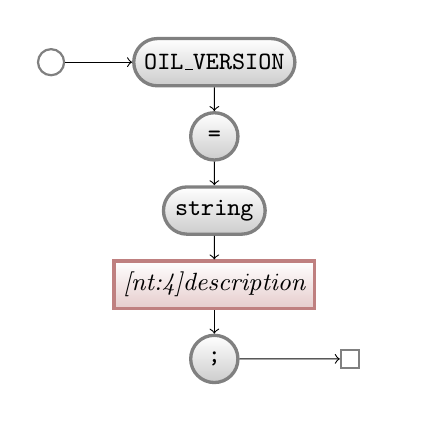
\begin{tikzpicture}
  \matrix[column sep=\ruleMatrixColumnSeparation, row sep=\ruleMatrixRowSeparation] {
    \node (P0start) [firstPoint] {}; & & \node (p4-2) [terminal] {OIL\_VERSION}; & \\
    & & \node (p3-2) [terminal] {=}; & \\
    & & \node (p2-2) [terminal] {string}; & \\
    & & \node (p1-2) [nonterminal] {\nonTerminalSymbol{description}{4}}; & \\
    & & \node (p0-2) [terminal] {;}; & \node (p0-3) [lastPoint] {}; & \\
  };
  \draw[->] (P0start) -- (p4-2) ;
  \draw[->] (p4-2) -- (p3-2) ;
  \draw[->] (p3-2) -- (p2-2) ;
  \draw[->] (p2-2) -- (p1-2) ;
  \draw[->] (p1-2) -- (p0-2) ;
  \draw[->] (p0-2) -- (p0-3) ;
\end{tikzpicture}

\nonTerminalSection{application\_definition}{6}

\ruleSubsection{goil\_syntax}{goil\_syntax}{170}

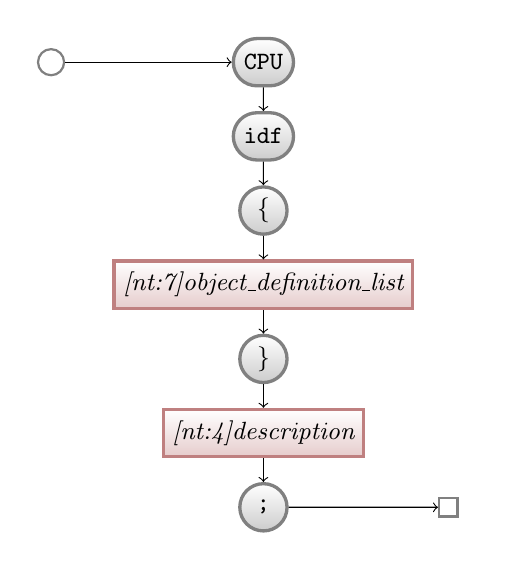
\begin{tikzpicture}
  \matrix[column sep=\ruleMatrixColumnSeparation, row sep=\ruleMatrixRowSeparation] {
    \node (P0start) [firstPoint] {}; & & \node (p6-2) [terminal] {CPU}; & \\
    & & \node (p5-2) [terminal] {idf}; & \\
    & & \node (p4-2) [terminal] {\{}; & \\
    & & \node (p3-2) [nonterminal] {\nonTerminalSymbol{object\_definition\_list}{7}}; & \\
    & & \node (p2-2) [terminal] {\}}; & \\
    & & \node (p1-2) [nonterminal] {\nonTerminalSymbol{description}{4}}; & \\
    & & \node (p0-2) [terminal] {;}; & \node (p0-3) [lastPoint] {}; & \\
  };
  \draw[->] (P0start) -- (p6-2) ;
  \draw[->] (p6-2) -- (p5-2) ;
  \draw[->] (p5-2) -- (p4-2) ;
  \draw[->] (p4-2) -- (p3-2) ;
  \draw[->] (p3-2) -- (p2-2) ;
  \draw[->] (p2-2) -- (p1-2) ;
  \draw[->] (p1-2) -- (p0-2) ;
  \draw[->] (p0-2) -- (p0-3) ;
\end{tikzpicture}

\nonTerminalSection{boolean}{8}

\ruleSubsection{goil\_syntax}{goil\_syntax}{234}

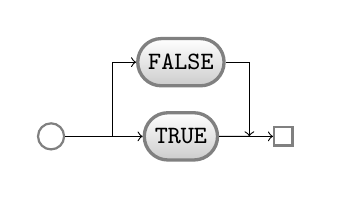
\begin{tikzpicture}
  \matrix[column sep=\ruleMatrixColumnSeparation, row sep=\ruleMatrixRowSeparation] {
    & & & \node (p1-3) [terminal] {FALSE}; & \\
    \node (P0start) [firstPoint] {}; & & \node (p0-2) [point] {}; & \node (p0-3) [terminal] {TRUE}; & \node (p0-4) [point] {}; & \node (p0-5) [lastPoint] {}; & \\
  };
  \draw[->] (P0start) -- (p0-3) ;
  \draw[->] (p0-2) |- (p1-3) ;
  \draw (p0-3) -- (p0-4) ;
  \draw[->] (p1-3) -| (p0-4) ;
  \draw[->] (p0-4) -- (p0-5) ;
\end{tikzpicture}

\nonTerminalSection{boolean\_options}{23}

\ruleSubsection{implementation\_parser}{implementation\_parser}{361}

\begin{tikzpicture}
  \matrix[column sep=\ruleMatrixColumnSeparation, row sep=\ruleMatrixRowSeparation] {
    & & & & \node (p2-4) [point] {}; & \\
    & & & & & & & \node (p1-7) [point] {}; & & & & & & & \node (p1-14) [point] {}; & & & & & & & & & \node (p1-23) [nonterminal] {\nonTerminalSymbol{description}{4}}; & \\
    \node (P0start) [firstPoint] {}; & & \node (p0-2) [nonterminal] {\nonTerminalSymbol{with\_auto}{28}}; & \node (p0-3) [point] {}; & \node (p0-4) [terminal] {[}; & \node (p0-5) [terminal] {TRUE}; & \node (p0-6) [point] {}; & \node (p0-7) [terminal] {\{}; & \node (p0-8) [nonterminal] {\nonTerminalSymbol{implementation\_list}{18}}; & \node (p0-9) [terminal] {\}}; & \node (p0-10) [point] {}; & \node (p0-11) [terminal] {,}; & \node (p0-12) [terminal] {FALSE}; & \node (p0-13) [point] {}; & \node (p0-14) [terminal] {\{}; & \node (p0-15) [nonterminal] {\nonTerminalSymbol{implementation\_list}{18}}; & \node (p0-16) [terminal] {\}}; & \node (p0-17) [point] {}; & \node (p0-18) [terminal] {]}; & \node (p0-19) [point] {}; & \node (p0-20) [nonterminal] {\nonTerminalSymbol{identifier\_or\_attribute}{34}}; & \node (p0-21) [nonterminal] {\nonTerminalSymbol{multiple}{33}}; & \node (p0-22) [point] {}; & \node (p0-23) [terminal] {=}; & \node (p0-24) [nonterminal] {\nonTerminalSymbol{boolean}{8}}; & \node (p0-25) [nonterminal] {\nonTerminalSymbol{description}{4}}; & \node (p0-26) [point] {}; & \node (p0-27) [lastPoint] {}; & \\
  };
  \draw[->] (P0start) -- (p0-2) ;
  \draw[->] (p0-2) -- (p0-4) ;
  \draw[->] (p0-4) -- (p0-5) ;
  \draw[->] (p0-5) -- (p0-7) ;
  \draw[->] (p0-7) -- (p0-8) ;
  \draw[->] (p0-8) -- (p0-9) ;
  \draw (p0-6) |- (p1-7) ;
  \draw (p0-9) -- (p0-10) ;
  \draw[->] (p1-7) -| (p0-10) ;
  \draw[->] (p0-10) -- (p0-11) ;
  \draw[->] (p0-11) -- (p0-12) ;
  \draw[->] (p0-12) -- (p0-14) ;
  \draw[->] (p0-14) -- (p0-15) ;
  \draw[->] (p0-15) -- (p0-16) ;
  \draw (p0-13) |- (p1-14) ;
  \draw (p0-16) -- (p0-17) ;
  \draw[->] (p1-14) -| (p0-17) ;
  \draw[->] (p0-17) -- (p0-18) ;
  \draw (p0-3) |- (p2-4) ;
  \draw (p0-18) -- (p0-19) ;
  \draw[->] (p2-4) -| (p0-19) ;
  \draw[->] (p0-19) -- (p0-20) ;
  \draw[->] (p0-20) -- (p0-21) ;
  \draw[->] (p0-21) -- (p0-23) ;
  \draw[->] (p0-23) -- (p0-24) ;
  \draw[->] (p0-24) -- (p0-25) ;
  \draw[->] (p0-22) |- (p1-23) ;
  \draw (p0-25) -- (p0-26) ;
  \draw[->] (p1-23) -| (p0-26) ;
  \draw[->] (p0-26) -- (p0-27) ;
\end{tikzpicture}

\nonTerminalSection{description}{4}

\ruleSubsection{goil\_syntax}{goil\_syntax}{139}

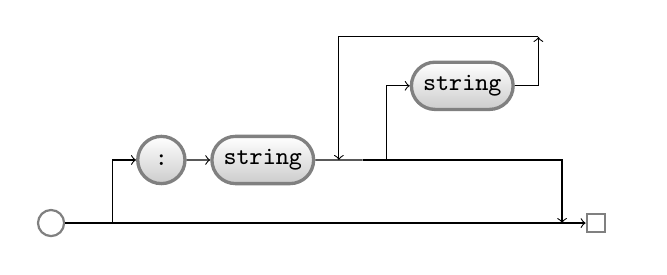
\begin{tikzpicture}
  \matrix[column sep=\ruleMatrixColumnSeparation, row sep=\ruleMatrixRowSeparation] {
    & & & & & & & & & \node (p3-9) [point] {}; & \\
    & & & & & & & & \node (p2-8) [terminal] {string}; & \\
    & & & \node (p1-3) [terminal] {:}; & \node (p1-4) [terminal] {string}; & \node (p1-5) [point] {}; & \node (p1-6) [point] {}; & \node (p1-7) [point] {}; & \\
    \node (P0start) [firstPoint] {}; & & \node (p0-2) [point] {}; & \node (p0-3) [point] {}; & & & & & & & \node (p0-10) [point] {}; & \node (p0-11) [lastPoint] {}; & \\
  };
  \draw (P0start) -- (p0-3) ;
  \draw[->] (p0-2) |- (p1-3) ;
  \draw[->] (p1-3) -- (p1-4) ;
  \draw (p1-4) -- (p1-6) ;
  \draw[->] (p1-7) |- (p2-8) ;
  \draw[->] (p3-9) -| (p1-5) ;
  \draw[->] (p2-8) -| (p3-9) ;
  \draw (p0-3) -- (p0-10) ;
  \draw[->] (p1-6) -| (p0-10) ;
  \draw[->] (p0-10) -- (p0-11) ;
\end{tikzpicture}

\nonTerminalSection{enum\_item}{24}

\ruleSubsection{implementation\_parser}{implementation\_parser}{406}

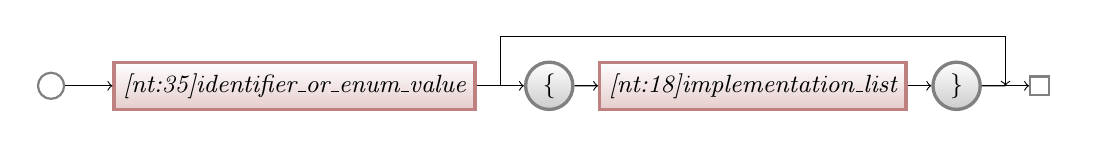
\begin{tikzpicture}
  \matrix[column sep=\ruleMatrixColumnSeparation, row sep=\ruleMatrixRowSeparation] {
    & & & & \node (p1-4) [point] {}; & \\
    \node (P0start) [firstPoint] {}; & & \node (p0-2) [nonterminal] {\nonTerminalSymbol{identifier\_or\_enum\_value}{35}}; & \node (p0-3) [point] {}; & \node (p0-4) [terminal] {\{}; & \node (p0-5) [nonterminal] {\nonTerminalSymbol{implementation\_list}{18}}; & \node (p0-6) [terminal] {\}}; & \node (p0-7) [point] {}; & \node (p0-8) [lastPoint] {}; & \\
  };
  \draw[->] (P0start) -- (p0-2) ;
  \draw[->] (p0-2) -- (p0-4) ;
  \draw[->] (p0-4) -- (p0-5) ;
  \draw[->] (p0-5) -- (p0-6) ;
  \draw (p0-3) |- (p1-4) ;
  \draw (p0-6) -- (p0-7) ;
  \draw[->] (p1-4) -| (p0-7) ;
  \draw[->] (p0-7) -- (p0-8) ;
\end{tikzpicture}

\nonTerminalSection{enum\_options}{25}

\ruleSubsection{implementation\_parser}{implementation\_parser}{419}

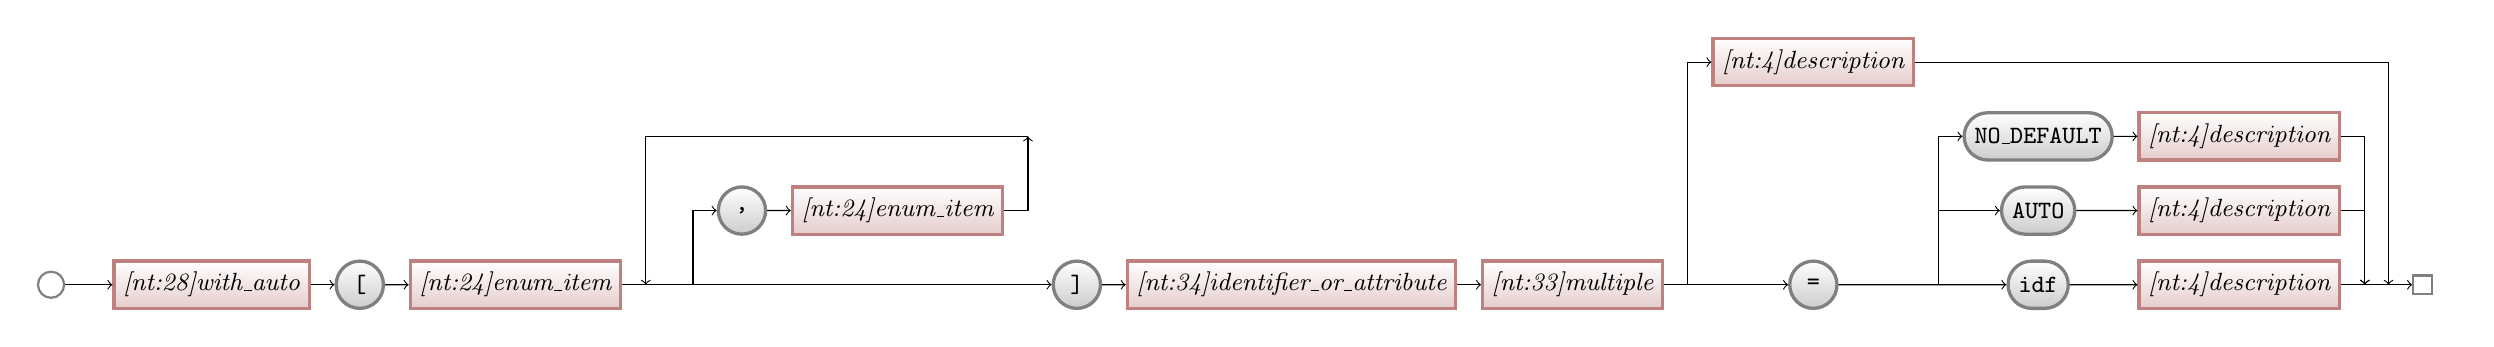
\begin{tikzpicture}
  \matrix[column sep=\ruleMatrixColumnSeparation, row sep=\ruleMatrixRowSeparation] {
    & & & & & & & & & & & & & & & \node (p3-15) [nonterminal] {\nonTerminalSymbol{description}{4}}; & \\
    & & & & & & & & & & \node (p2-10) [point] {}; & & & & & & & \node (p2-17) [terminal] {NO\_DEFAULT}; & \node (p2-18) [nonterminal] {\nonTerminalSymbol{description}{4}}; & \\
    & & & & & & & & \node (p1-8) [terminal] {,}; & \node (p1-9) [nonterminal] {\nonTerminalSymbol{enum\_item}{24}}; & & & & & & & & \node (p1-17) [terminal] {AUTO}; & \node (p1-18) [nonterminal] {\nonTerminalSymbol{description}{4}}; & \\
    \node (P0start) [firstPoint] {}; & & \node (p0-2) [nonterminal] {\nonTerminalSymbol{with\_auto}{28}}; & \node (p0-3) [terminal] {[}; & \node (p0-4) [nonterminal] {\nonTerminalSymbol{enum\_item}{24}}; & \node (p0-5) [point] {}; & \node (p0-6) [point] {}; & \node (p0-7) [point] {}; & & & & \node (p0-11) [terminal] {]}; & \node (p0-12) [nonterminal] {\nonTerminalSymbol{identifier\_or\_attribute}{34}}; & \node (p0-13) [nonterminal] {\nonTerminalSymbol{multiple}{33}}; & \node (p0-14) [point] {}; & \node (p0-15) [terminal] {=}; & \node (p0-16) [point] {}; & \node (p0-17) [terminal] {idf}; & \node (p0-18) [nonterminal] {\nonTerminalSymbol{description}{4}}; & \node (p0-19) [point] {}; & \node (p0-20) [point] {}; & \node (p0-21) [lastPoint] {}; & \\
  };
  \draw[->] (P0start) -- (p0-2) ;
  \draw[->] (p0-2) -- (p0-3) ;
  \draw[->] (p0-3) -- (p0-4) ;
  \draw (p0-4) -- (p0-6) ;
  \draw[->] (p0-7) |- (p1-8) ;
  \draw[->] (p1-8) -- (p1-9) ;
  \draw[->] (p2-10) -| (p0-5) ;
  \draw[->] (p1-9) -| (p2-10) ;
  \draw[->] (p0-6) -- (p0-11) ;
  \draw[->] (p0-11) -- (p0-12) ;
  \draw[->] (p0-12) -- (p0-13) ;
  \draw[->] (p0-13) -- (p0-15) ;
  \draw[->] (p0-15) -- (p0-17) ;
  \draw[->] (p0-17) -- (p0-18) ;
  \draw[->] (p0-16) |- (p1-17) ;
  \draw[->] (p1-17) -- (p1-18) ;
  \draw[->] (p0-16) |- (p2-17) ;
  \draw[->] (p2-17) -- (p2-18) ;
  \draw (p0-18) -- (p0-19) ;
  \draw[->] (p1-18) -| (p0-19) ;
  \draw[->] (p2-18) -| (p0-19) ;
  \draw[->] (p0-14) |- (p3-15) ;
  \draw (p0-19) -- (p0-20) ;
  \draw[->] (p3-15) -| (p0-20) ;
  \draw[->] (p0-20) -- (p0-21) ;
\end{tikzpicture}

\nonTerminalSection{file}{2}

\ruleSubsection{goil\_syntax}{goil\_syntax}{110}

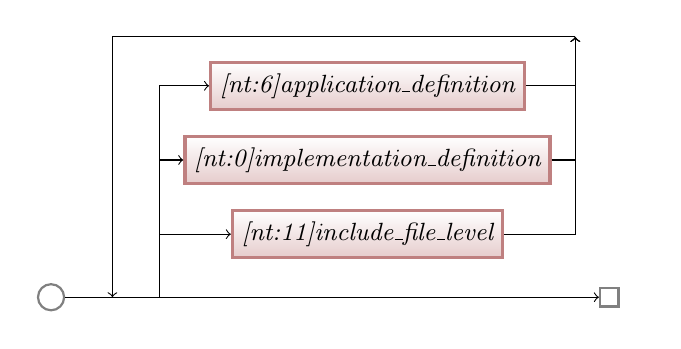
\begin{tikzpicture}
  \matrix[column sep=\ruleMatrixColumnSeparation, row sep=\ruleMatrixRowSeparation] {
    & & & & & & \node (p4-6) [point] {}; & \\
    & & & & & \node (p3-5) [nonterminal] {\nonTerminalSymbol{application\_definition}{6}}; & \\
    & & & & & \node (p2-5) [nonterminal] {\nonTerminalSymbol{implementation\_definition}{0}}; & \\
    & & & & & \node (p1-5) [nonterminal] {\nonTerminalSymbol{include\_file\_level}{11}}; & \\
    \node (P0start) [firstPoint] {}; & & \node (p0-2) [point] {}; & \node (p0-3) [point] {}; & \node (p0-4) [point] {}; & & & \node (p0-7) [lastPoint] {}; & \\
  };
  \draw (P0start) -- (p0-3) ;
  \draw[->] (p0-4) |- (p1-5) ;
  \draw[->] (p0-4) |- (p2-5) ;
  \draw[->] (p0-4) |- (p3-5) ;
  \draw[->] (p4-6) -| (p0-2) ;
  \draw[->] (p1-5) -| (p4-6) ;
  \draw[->] (p2-5) -| (p4-6) ;
  \draw[->] (p3-5) -| (p4-6) ;
  \draw[->] (p0-3) -- (p0-7) ;
\end{tikzpicture}

\nonTerminalSection{identifier\_or\_attribute}{34}

\ruleSubsection{implementation\_parser}{implementation\_parser}{643}

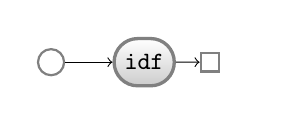
\begin{tikzpicture}
  \matrix[column sep=\ruleMatrixColumnSeparation, row sep=\ruleMatrixRowSeparation] {
    \node (P0start) [firstPoint] {}; & & \node (p0-2) [terminal] {idf}; & \node (p0-3) [lastPoint] {}; & \\
  };
  \draw[->] (P0start) -- (p0-2) ;
  \draw[->] (p0-2) -- (p0-3) ;
\end{tikzpicture}

\nonTerminalSection{identifier\_or\_enum\_value}{35}

\ruleSubsection{implementation\_parser}{implementation\_parser}{648}

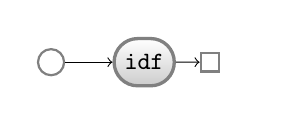
\begin{tikzpicture}
  \matrix[column sep=\ruleMatrixColumnSeparation, row sep=\ruleMatrixRowSeparation] {
    \node (P0start) [firstPoint] {}; & & \node (p0-2) [terminal] {idf}; & \node (p0-3) [lastPoint] {}; & \\
  };
  \draw[->] (P0start) -- (p0-2) ;
  \draw[->] (p0-2) -- (p0-3) ;
\end{tikzpicture}

\nonTerminalSection{implementation\_definition}{0}

\ruleSubsection{implementation\_parser}{implementation\_parser}{55}

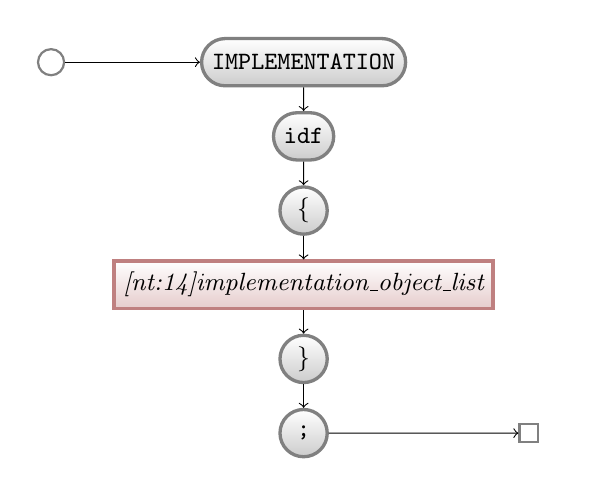
\begin{tikzpicture}
  \matrix[column sep=\ruleMatrixColumnSeparation, row sep=\ruleMatrixRowSeparation] {
    \node (P0start) [firstPoint] {}; & & \node (p5-2) [terminal] {IMPLEMENTATION}; & \\
    & & \node (p4-2) [terminal] {idf}; & \\
    & & \node (p3-2) [terminal] {\{}; & \\
    & & \node (p2-2) [nonterminal] {\nonTerminalSymbol{implementation\_object\_list}{14}}; & \\
    & & \node (p1-2) [terminal] {\}}; & \\
    & & \node (p0-2) [terminal] {;}; & \node (p0-3) [lastPoint] {}; & \\
  };
  \draw[->] (P0start) -- (p5-2) ;
  \draw[->] (p5-2) -- (p4-2) ;
  \draw[->] (p4-2) -- (p3-2) ;
  \draw[->] (p3-2) -- (p2-2) ;
  \draw[->] (p2-2) -- (p1-2) ;
  \draw[->] (p1-2) -- (p0-2) ;
  \draw[->] (p0-2) -- (p0-3) ;
\end{tikzpicture}

\nonTerminalSection{implementation\_list}{18}

\ruleSubsection{implementation\_parser}{implementation\_parser}{183}

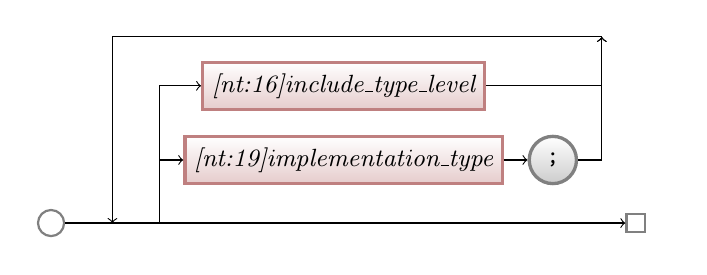
\begin{tikzpicture}
  \matrix[column sep=\ruleMatrixColumnSeparation, row sep=\ruleMatrixRowSeparation] {
    & & & & & & & \node (p3-7) [point] {}; & \\
    & & & & & \node (p2-5) [nonterminal] {\nonTerminalSymbol{include\_type\_level}{16}}; & \\
    & & & & & \node (p1-5) [nonterminal] {\nonTerminalSymbol{implementation\_type}{19}}; & \node (p1-6) [terminal] {;}; & \\
    \node (P0start) [firstPoint] {}; & & \node (p0-2) [point] {}; & \node (p0-3) [point] {}; & \node (p0-4) [point] {}; & & & & \node (p0-8) [lastPoint] {}; & \\
  };
  \draw (P0start) -- (p0-3) ;
  \draw[->] (p0-4) |- (p1-5) ;
  \draw[->] (p1-5) -- (p1-6) ;
  \draw[->] (p0-4) |- (p2-5) ;
  \draw[->] (p3-7) -| (p0-2) ;
  \draw[->] (p1-6) -| (p3-7) ;
  \draw[->] (p2-5) -| (p3-7) ;
  \draw[->] (p0-3) -- (p0-8) ;
\end{tikzpicture}

\nonTerminalSection{implementation\_object\_list}{14}

\ruleSubsection{implementation\_parser}{implementation\_parser}{62}

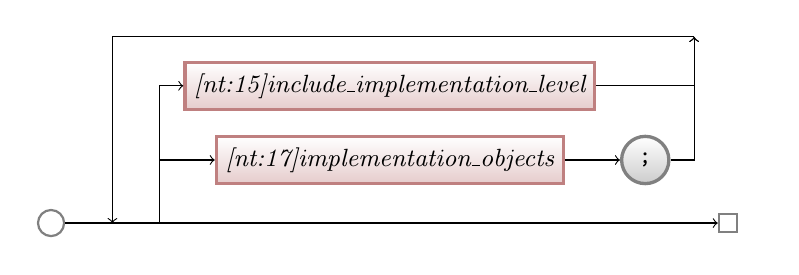
\begin{tikzpicture}
  \matrix[column sep=\ruleMatrixColumnSeparation, row sep=\ruleMatrixRowSeparation] {
    & & & & & & & \node (p3-7) [point] {}; & \\
    & & & & & \node (p2-5) [nonterminal] {\nonTerminalSymbol{include\_implementation\_level}{15}}; & \\
    & & & & & \node (p1-5) [nonterminal] {\nonTerminalSymbol{implementation\_objects}{17}}; & \node (p1-6) [terminal] {;}; & \\
    \node (P0start) [firstPoint] {}; & & \node (p0-2) [point] {}; & \node (p0-3) [point] {}; & \node (p0-4) [point] {}; & & & & \node (p0-8) [lastPoint] {}; & \\
  };
  \draw (P0start) -- (p0-3) ;
  \draw[->] (p0-4) |- (p1-5) ;
  \draw[->] (p1-5) -- (p1-6) ;
  \draw[->] (p0-4) |- (p2-5) ;
  \draw[->] (p3-7) -| (p0-2) ;
  \draw[->] (p1-6) -| (p3-7) ;
  \draw[->] (p2-5) -| (p3-7) ;
  \draw[->] (p0-3) -- (p0-8) ;
\end{tikzpicture}

\nonTerminalSection{implementation\_objects}{17}

\ruleSubsection{implementation\_parser}{implementation\_parser}{135}

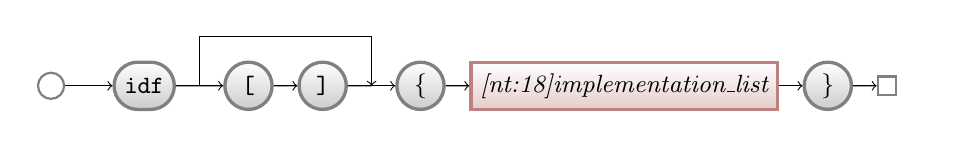
\begin{tikzpicture}
  \matrix[column sep=\ruleMatrixColumnSeparation, row sep=\ruleMatrixRowSeparation] {
    & & & & \node (p1-4) [point] {}; & \\
    \node (P0start) [firstPoint] {}; & & \node (p0-2) [terminal] {idf}; & \node (p0-3) [point] {}; & \node (p0-4) [terminal] {[}; & \node (p0-5) [terminal] {]}; & \node (p0-6) [point] {}; & \node (p0-7) [terminal] {\{}; & \node (p0-8) [nonterminal] {\nonTerminalSymbol{implementation\_list}{18}}; & \node (p0-9) [terminal] {\}}; & \node (p0-10) [lastPoint] {}; & \\
  };
  \draw[->] (P0start) -- (p0-2) ;
  \draw[->] (p0-2) -- (p0-4) ;
  \draw[->] (p0-4) -- (p0-5) ;
  \draw (p0-3) |- (p1-4) ;
  \draw (p0-5) -- (p0-6) ;
  \draw[->] (p1-4) -| (p0-6) ;
  \draw[->] (p0-6) -- (p0-7) ;
  \draw[->] (p0-7) -- (p0-8) ;
  \draw[->] (p0-8) -- (p0-9) ;
  \draw[->] (p0-9) -- (p0-10) ;
\end{tikzpicture}

\nonTerminalSection{implementation\_type}{19}

\ruleSubsection{implementation\_parser}{implementation\_parser}{261}

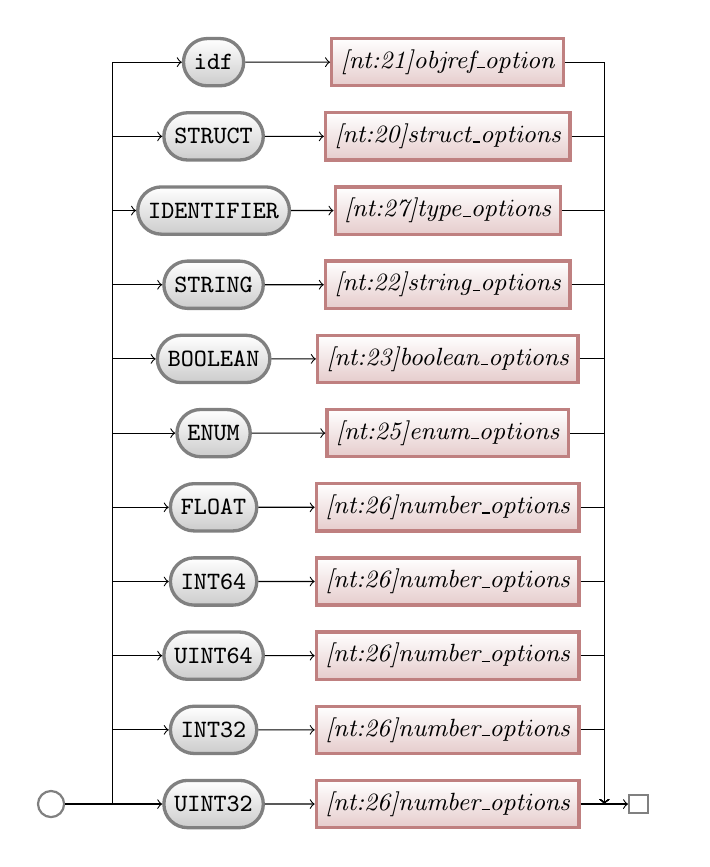
\begin{tikzpicture}
  \matrix[column sep=\ruleMatrixColumnSeparation, row sep=\ruleMatrixRowSeparation] {
    & & & \node (p10-3) [terminal] {idf}; & \node (p10-4) [nonterminal] {\nonTerminalSymbol{objref\_option}{21}}; & \\
    & & & \node (p9-3) [terminal] {STRUCT}; & \node (p9-4) [nonterminal] {\nonTerminalSymbol{struct\_options}{20}}; & \\
    & & & \node (p8-3) [terminal] {IDENTIFIER}; & \node (p8-4) [nonterminal] {\nonTerminalSymbol{type\_options}{27}}; & \\
    & & & \node (p7-3) [terminal] {STRING}; & \node (p7-4) [nonterminal] {\nonTerminalSymbol{string\_options}{22}}; & \\
    & & & \node (p6-3) [terminal] {BOOLEAN}; & \node (p6-4) [nonterminal] {\nonTerminalSymbol{boolean\_options}{23}}; & \\
    & & & \node (p5-3) [terminal] {ENUM}; & \node (p5-4) [nonterminal] {\nonTerminalSymbol{enum\_options}{25}}; & \\
    & & & \node (p4-3) [terminal] {FLOAT}; & \node (p4-4) [nonterminal] {\nonTerminalSymbol{number\_options}{26}}; & \\
    & & & \node (p3-3) [terminal] {INT64}; & \node (p3-4) [nonterminal] {\nonTerminalSymbol{number\_options}{26}}; & \\
    & & & \node (p2-3) [terminal] {UINT64}; & \node (p2-4) [nonterminal] {\nonTerminalSymbol{number\_options}{26}}; & \\
    & & & \node (p1-3) [terminal] {INT32}; & \node (p1-4) [nonterminal] {\nonTerminalSymbol{number\_options}{26}}; & \\
    \node (P0start) [firstPoint] {}; & & \node (p0-2) [point] {}; & \node (p0-3) [terminal] {UINT32}; & \node (p0-4) [nonterminal] {\nonTerminalSymbol{number\_options}{26}}; & \node (p0-5) [point] {}; & \node (p0-6) [lastPoint] {}; & \\
  };
  \draw[->] (P0start) -- (p0-3) ;
  \draw[->] (p0-3) -- (p0-4) ;
  \draw[->] (p0-2) |- (p1-3) ;
  \draw[->] (p1-3) -- (p1-4) ;
  \draw[->] (p0-2) |- (p2-3) ;
  \draw[->] (p2-3) -- (p2-4) ;
  \draw[->] (p0-2) |- (p3-3) ;
  \draw[->] (p3-3) -- (p3-4) ;
  \draw[->] (p0-2) |- (p4-3) ;
  \draw[->] (p4-3) -- (p4-4) ;
  \draw[->] (p0-2) |- (p5-3) ;
  \draw[->] (p5-3) -- (p5-4) ;
  \draw[->] (p0-2) |- (p6-3) ;
  \draw[->] (p6-3) -- (p6-4) ;
  \draw[->] (p0-2) |- (p7-3) ;
  \draw[->] (p7-3) -- (p7-4) ;
  \draw[->] (p0-2) |- (p8-3) ;
  \draw[->] (p8-3) -- (p8-4) ;
  \draw[->] (p0-2) |- (p9-3) ;
  \draw[->] (p9-3) -- (p9-4) ;
  \draw[->] (p0-2) |- (p10-3) ;
  \draw[->] (p10-3) -- (p10-4) ;
  \draw (p0-4) -- (p0-5) ;
  \draw[->] (p1-4) -| (p0-5) ;
  \draw[->] (p2-4) -| (p0-5) ;
  \draw[->] (p3-4) -| (p0-5) ;
  \draw[->] (p4-4) -| (p0-5) ;
  \draw[->] (p5-4) -| (p0-5) ;
  \draw[->] (p6-4) -| (p0-5) ;
  \draw[->] (p7-4) -| (p0-5) ;
  \draw[->] (p8-4) -| (p0-5) ;
  \draw[->] (p9-4) -| (p0-5) ;
  \draw[->] (p10-4) -| (p0-5) ;
  \draw[->] (p0-5) -- (p0-6) ;
\end{tikzpicture}

\nonTerminalSection{include\_cpu\_level}{12}

\ruleSubsection{goil\_syntax}{goil\_syntax}{475}

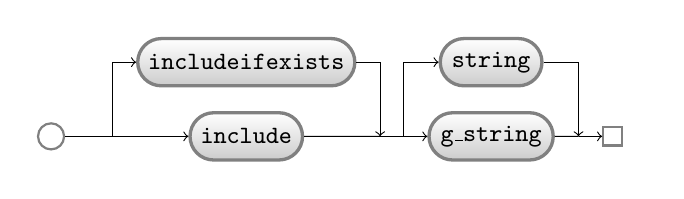
\begin{tikzpicture}
  \matrix[column sep=\ruleMatrixColumnSeparation, row sep=\ruleMatrixRowSeparation] {
    & & & \node (p1-3) [terminal] {includeifexists}; & & & \node (p1-6) [terminal] {string}; & \\
    \node (P0start) [firstPoint] {}; & & \node (p0-2) [point] {}; & \node (p0-3) [terminal] {include}; & \node (p0-4) [point] {}; & \node (p0-5) [point] {}; & \node (p0-6) [terminal] {g\_string}; & \node (p0-7) [point] {}; & \node (p0-8) [lastPoint] {}; & \\
  };
  \draw[->] (P0start) -- (p0-3) ;
  \draw[->] (p0-2) |- (p1-3) ;
  \draw (p0-3) -- (p0-4) ;
  \draw[->] (p1-3) -| (p0-4) ;
  \draw[->] (p0-4) -- (p0-6) ;
  \draw[->] (p0-5) |- (p1-6) ;
  \draw (p0-6) -- (p0-7) ;
  \draw[->] (p1-6) -| (p0-7) ;
  \draw[->] (p0-7) -- (p0-8) ;
\end{tikzpicture}

\nonTerminalSection{include\_file\_level}{11}

\ruleSubsection{goil\_syntax}{goil\_syntax}{451}

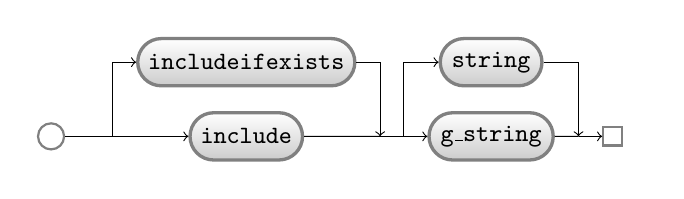
\begin{tikzpicture}
  \matrix[column sep=\ruleMatrixColumnSeparation, row sep=\ruleMatrixRowSeparation] {
    & & & \node (p1-3) [terminal] {includeifexists}; & & & \node (p1-6) [terminal] {string}; & \\
    \node (P0start) [firstPoint] {}; & & \node (p0-2) [point] {}; & \node (p0-3) [terminal] {include}; & \node (p0-4) [point] {}; & \node (p0-5) [point] {}; & \node (p0-6) [terminal] {g\_string}; & \node (p0-7) [point] {}; & \node (p0-8) [lastPoint] {}; & \\
  };
  \draw[->] (P0start) -- (p0-3) ;
  \draw[->] (p0-2) |- (p1-3) ;
  \draw (p0-3) -- (p0-4) ;
  \draw[->] (p1-3) -| (p0-4) ;
  \draw[->] (p0-4) -- (p0-6) ;
  \draw[->] (p0-5) |- (p1-6) ;
  \draw (p0-6) -- (p0-7) ;
  \draw[->] (p1-6) -| (p0-7) ;
  \draw[->] (p0-7) -- (p0-8) ;
\end{tikzpicture}

\nonTerminalSection{include\_implementation\_level}{15}

\ruleSubsection{implementation\_parser}{implementation\_parser}{71}

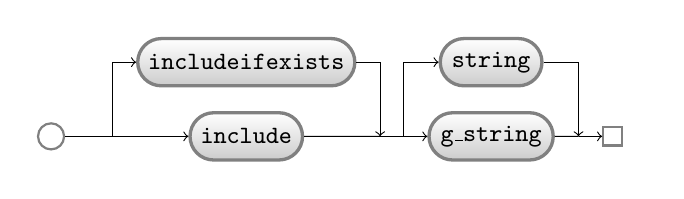
\begin{tikzpicture}
  \matrix[column sep=\ruleMatrixColumnSeparation, row sep=\ruleMatrixRowSeparation] {
    & & & \node (p1-3) [terminal] {includeifexists}; & & & \node (p1-6) [terminal] {string}; & \\
    \node (P0start) [firstPoint] {}; & & \node (p0-2) [point] {}; & \node (p0-3) [terminal] {include}; & \node (p0-4) [point] {}; & \node (p0-5) [point] {}; & \node (p0-6) [terminal] {g\_string}; & \node (p0-7) [point] {}; & \node (p0-8) [lastPoint] {}; & \\
  };
  \draw[->] (P0start) -- (p0-3) ;
  \draw[->] (p0-2) |- (p1-3) ;
  \draw (p0-3) -- (p0-4) ;
  \draw[->] (p1-3) -| (p0-4) ;
  \draw[->] (p0-4) -- (p0-6) ;
  \draw[->] (p0-5) |- (p1-6) ;
  \draw (p0-6) -- (p0-7) ;
  \draw[->] (p1-6) -| (p0-7) ;
  \draw[->] (p0-7) -- (p0-8) ;
\end{tikzpicture}

\nonTerminalSection{include\_object\_level}{13}

\ruleSubsection{goil\_syntax}{goil\_syntax}{499}

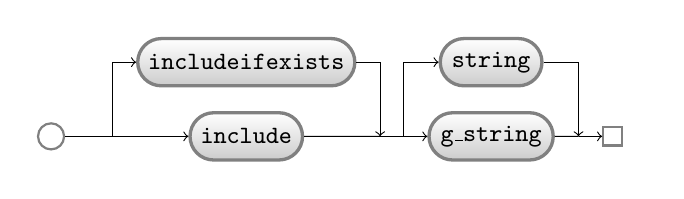
\begin{tikzpicture}
  \matrix[column sep=\ruleMatrixColumnSeparation, row sep=\ruleMatrixRowSeparation] {
    & & & \node (p1-3) [terminal] {includeifexists}; & & & \node (p1-6) [terminal] {string}; & \\
    \node (P0start) [firstPoint] {}; & & \node (p0-2) [point] {}; & \node (p0-3) [terminal] {include}; & \node (p0-4) [point] {}; & \node (p0-5) [point] {}; & \node (p0-6) [terminal] {g\_string}; & \node (p0-7) [point] {}; & \node (p0-8) [lastPoint] {}; & \\
  };
  \draw[->] (P0start) -- (p0-3) ;
  \draw[->] (p0-2) |- (p1-3) ;
  \draw (p0-3) -- (p0-4) ;
  \draw[->] (p1-3) -| (p0-4) ;
  \draw[->] (p0-4) -- (p0-6) ;
  \draw[->] (p0-5) |- (p1-6) ;
  \draw (p0-6) -- (p0-7) ;
  \draw[->] (p1-6) -| (p0-7) ;
  \draw[->] (p0-7) -- (p0-8) ;
\end{tikzpicture}

\nonTerminalSection{include\_type\_level}{16}

\ruleSubsection{implementation\_parser}{implementation\_parser}{92}

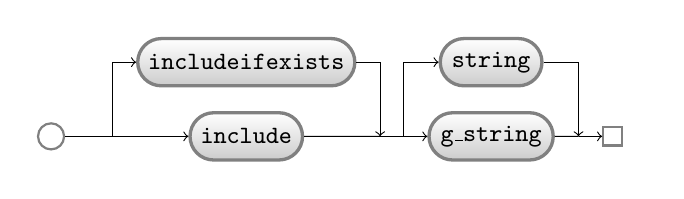
\begin{tikzpicture}
  \matrix[column sep=\ruleMatrixColumnSeparation, row sep=\ruleMatrixRowSeparation] {
    & & & \node (p1-3) [terminal] {includeifexists}; & & & \node (p1-6) [terminal] {string}; & \\
    \node (P0start) [firstPoint] {}; & & \node (p0-2) [point] {}; & \node (p0-3) [terminal] {include}; & \node (p0-4) [point] {}; & \node (p0-5) [point] {}; & \node (p0-6) [terminal] {g\_string}; & \node (p0-7) [point] {}; & \node (p0-8) [lastPoint] {}; & \\
  };
  \draw[->] (P0start) -- (p0-3) ;
  \draw[->] (p0-2) |- (p1-3) ;
  \draw (p0-3) -- (p0-4) ;
  \draw[->] (p1-3) -| (p0-4) ;
  \draw[->] (p0-4) -- (p0-6) ;
  \draw[->] (p0-5) |- (p1-6) ;
  \draw (p0-6) -- (p0-7) ;
  \draw[->] (p1-6) -| (p0-7) ;
  \draw[->] (p0-7) -- (p0-8) ;
\end{tikzpicture}

\nonTerminalSection{int\_or\_float}{29}

\ruleSubsection{implementation\_parser}{implementation\_parser}{553}

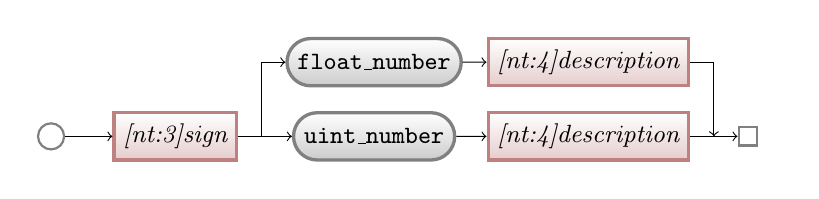
\begin{tikzpicture}
  \matrix[column sep=\ruleMatrixColumnSeparation, row sep=\ruleMatrixRowSeparation] {
    & & & & \node (p1-4) [terminal] {float\_number}; & \node (p1-5) [nonterminal] {\nonTerminalSymbol{description}{4}}; & \\
    \node (P0start) [firstPoint] {}; & & \node (p0-2) [nonterminal] {\nonTerminalSymbol{sign}{3}}; & \node (p0-3) [point] {}; & \node (p0-4) [terminal] {uint\_number}; & \node (p0-5) [nonterminal] {\nonTerminalSymbol{description}{4}}; & \node (p0-6) [point] {}; & \node (p0-7) [lastPoint] {}; & \\
  };
  \draw[->] (P0start) -- (p0-2) ;
  \draw[->] (p0-2) -- (p0-4) ;
  \draw[->] (p0-4) -- (p0-5) ;
  \draw[->] (p0-3) |- (p1-4) ;
  \draw[->] (p1-4) -- (p1-5) ;
  \draw (p0-5) -- (p0-6) ;
  \draw[->] (p1-5) -| (p0-6) ;
  \draw[->] (p0-6) -- (p0-7) ;
\end{tikzpicture}

\nonTerminalSection{multiple}{33}

\ruleSubsection{implementation\_parser}{implementation\_parser}{633}

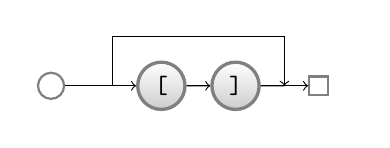
\begin{tikzpicture}
  \matrix[column sep=\ruleMatrixColumnSeparation, row sep=\ruleMatrixRowSeparation] {
    & & & \node (p1-3) [point] {}; & \\
    \node (P0start) [firstPoint] {}; & & \node (p0-2) [point] {}; & \node (p0-3) [terminal] {[}; & \node (p0-4) [terminal] {]}; & \node (p0-5) [point] {}; & \node (p0-6) [lastPoint] {}; & \\
  };
  \draw[->] (P0start) -- (p0-3) ;
  \draw[->] (p0-3) -- (p0-4) ;
  \draw (p0-2) |- (p1-3) ;
  \draw (p0-4) -- (p0-5) ;
  \draw[->] (p1-3) -| (p0-5) ;
  \draw[->] (p0-5) -- (p0-6) ;
\end{tikzpicture}

\nonTerminalSection{number\_options}{26}

\ruleSubsection{implementation\_parser}{implementation\_parser}{466}

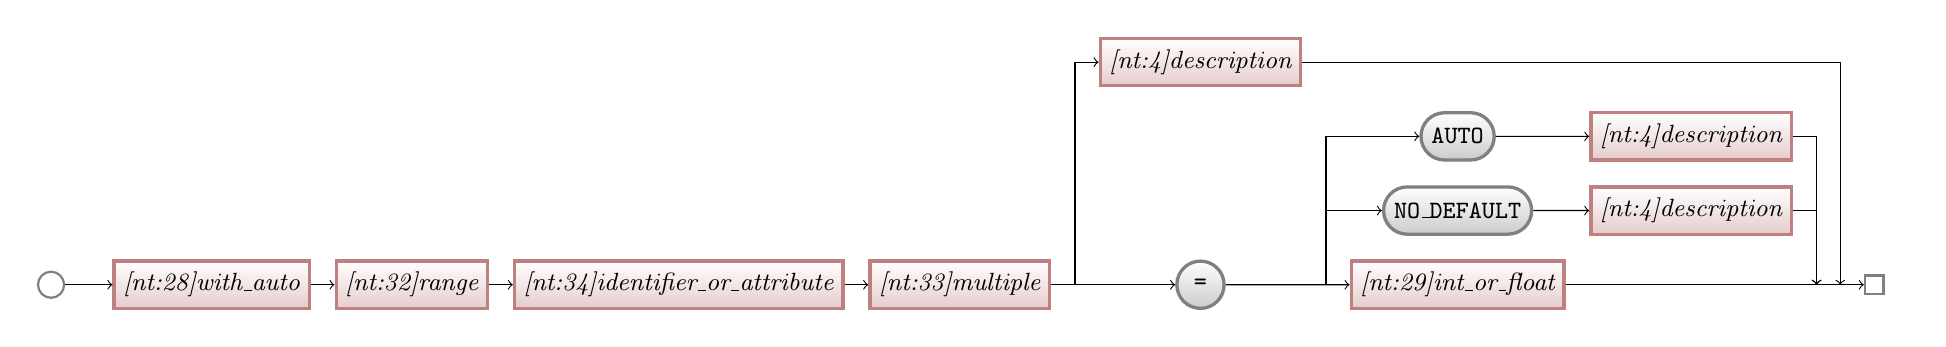
\begin{tikzpicture}
  \matrix[column sep=\ruleMatrixColumnSeparation, row sep=\ruleMatrixRowSeparation] {
    & & & & & & & \node (p3-7) [nonterminal] {\nonTerminalSymbol{description}{4}}; & \\
    & & & & & & & & & \node (p2-9) [terminal] {AUTO}; & \node (p2-10) [nonterminal] {\nonTerminalSymbol{description}{4}}; & \\
    & & & & & & & & & \node (p1-9) [terminal] {NO\_DEFAULT}; & \node (p1-10) [nonterminal] {\nonTerminalSymbol{description}{4}}; & \\
    \node (P0start) [firstPoint] {}; & & \node (p0-2) [nonterminal] {\nonTerminalSymbol{with\_auto}{28}}; & \node (p0-3) [nonterminal] {\nonTerminalSymbol{range}{32}}; & \node (p0-4) [nonterminal] {\nonTerminalSymbol{identifier\_or\_attribute}{34}}; & \node (p0-5) [nonterminal] {\nonTerminalSymbol{multiple}{33}}; & \node (p0-6) [point] {}; & \node (p0-7) [terminal] {=}; & \node (p0-8) [point] {}; & \node (p0-9) [nonterminal] {\nonTerminalSymbol{int\_or\_float}{29}}; & & \node (p0-11) [point] {}; & \node (p0-12) [point] {}; & \node (p0-13) [lastPoint] {}; & \\
  };
  \draw[->] (P0start) -- (p0-2) ;
  \draw[->] (p0-2) -- (p0-3) ;
  \draw[->] (p0-3) -- (p0-4) ;
  \draw[->] (p0-4) -- (p0-5) ;
  \draw[->] (p0-5) -- (p0-7) ;
  \draw[->] (p0-7) -- (p0-9) ;
  \draw[->] (p0-8) |- (p1-9) ;
  \draw[->] (p1-9) -- (p1-10) ;
  \draw[->] (p0-8) |- (p2-9) ;
  \draw[->] (p2-9) -- (p2-10) ;
  \draw (p0-9) -- (p0-11) ;
  \draw[->] (p1-10) -| (p0-11) ;
  \draw[->] (p2-10) -| (p0-11) ;
  \draw[->] (p0-6) |- (p3-7) ;
  \draw (p0-11) -- (p0-12) ;
  \draw[->] (p3-7) -| (p0-12) ;
  \draw[->] (p0-12) -- (p0-13) ;
\end{tikzpicture}

\nonTerminalSection{object\_definition\_list}{7}

\ruleSubsection{goil\_syntax}{goil\_syntax}{184}

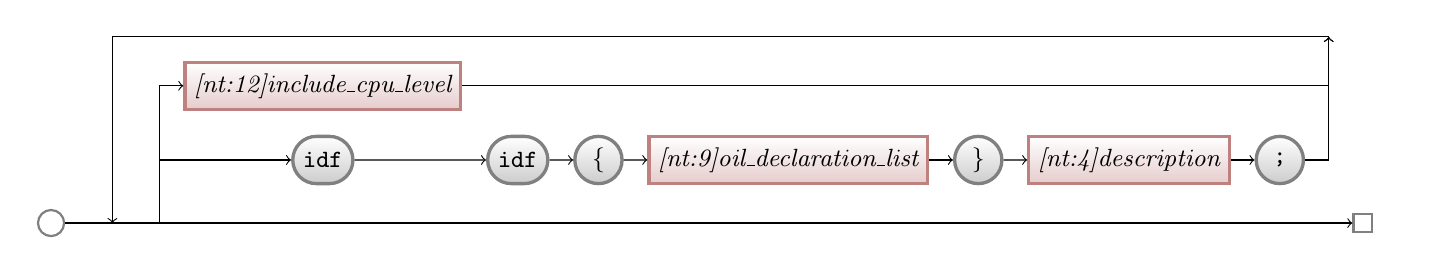
\begin{tikzpicture}
  \matrix[column sep=\ruleMatrixColumnSeparation, row sep=\ruleMatrixRowSeparation] {
    & & & & & & & & & & & & \node (p3-12) [point] {}; & \\
    & & & & & \node (p2-5) [nonterminal] {\nonTerminalSymbol{include\_cpu\_level}{12}}; & \\
    & & & & & \node (p1-5) [terminal] {idf}; & \node (p1-6) [terminal] {idf}; & \node (p1-7) [terminal] {\{}; & \node (p1-8) [nonterminal] {\nonTerminalSymbol{oil\_declaration\_list}{9}}; & \node (p1-9) [terminal] {\}}; & \node (p1-10) [nonterminal] {\nonTerminalSymbol{description}{4}}; & \node (p1-11) [terminal] {;}; & \\
    \node (P0start) [firstPoint] {}; & & \node (p0-2) [point] {}; & \node (p0-3) [point] {}; & \node (p0-4) [point] {}; & & & & & & & & & \node (p0-13) [lastPoint] {}; & \\
  };
  \draw (P0start) -- (p0-3) ;
  \draw[->] (p0-4) |- (p1-5) ;
  \draw[->] (p1-5) -- (p1-6) ;
  \draw[->] (p1-6) -- (p1-7) ;
  \draw[->] (p1-7) -- (p1-8) ;
  \draw[->] (p1-8) -- (p1-9) ;
  \draw[->] (p1-9) -- (p1-10) ;
  \draw[->] (p1-10) -- (p1-11) ;
  \draw[->] (p0-4) |- (p2-5) ;
  \draw[->] (p3-12) -| (p0-2) ;
  \draw[->] (p1-11) -| (p3-12) ;
  \draw[->] (p2-5) -| (p3-12) ;
  \draw[->] (p0-3) -- (p0-13) ;
\end{tikzpicture}

\nonTerminalSection{objref\_option}{21}

\ruleSubsection{implementation\_parser}{implementation\_parser}{306}

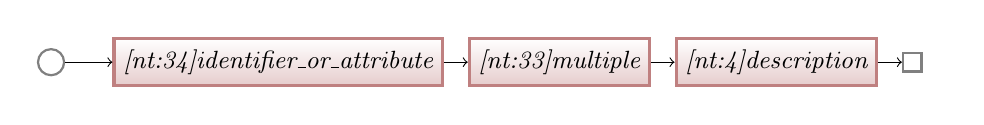
\begin{tikzpicture}
  \matrix[column sep=\ruleMatrixColumnSeparation, row sep=\ruleMatrixRowSeparation] {
    \node (P0start) [firstPoint] {}; & & \node (p0-2) [nonterminal] {\nonTerminalSymbol{identifier\_or\_attribute}{34}}; & \node (p0-3) [nonterminal] {\nonTerminalSymbol{multiple}{33}}; & \node (p0-4) [nonterminal] {\nonTerminalSymbol{description}{4}}; & \node (p0-5) [lastPoint] {}; & \\
  };
  \draw[->] (P0start) -- (p0-2) ;
  \draw[->] (p0-2) -- (p0-3) ;
  \draw[->] (p0-3) -- (p0-4) ;
  \draw[->] (p0-4) -- (p0-5) ;
\end{tikzpicture}

\nonTerminalSection{oil\_declaration}{10}

\ruleSubsection{goil\_syntax}{goil\_syntax}{256}

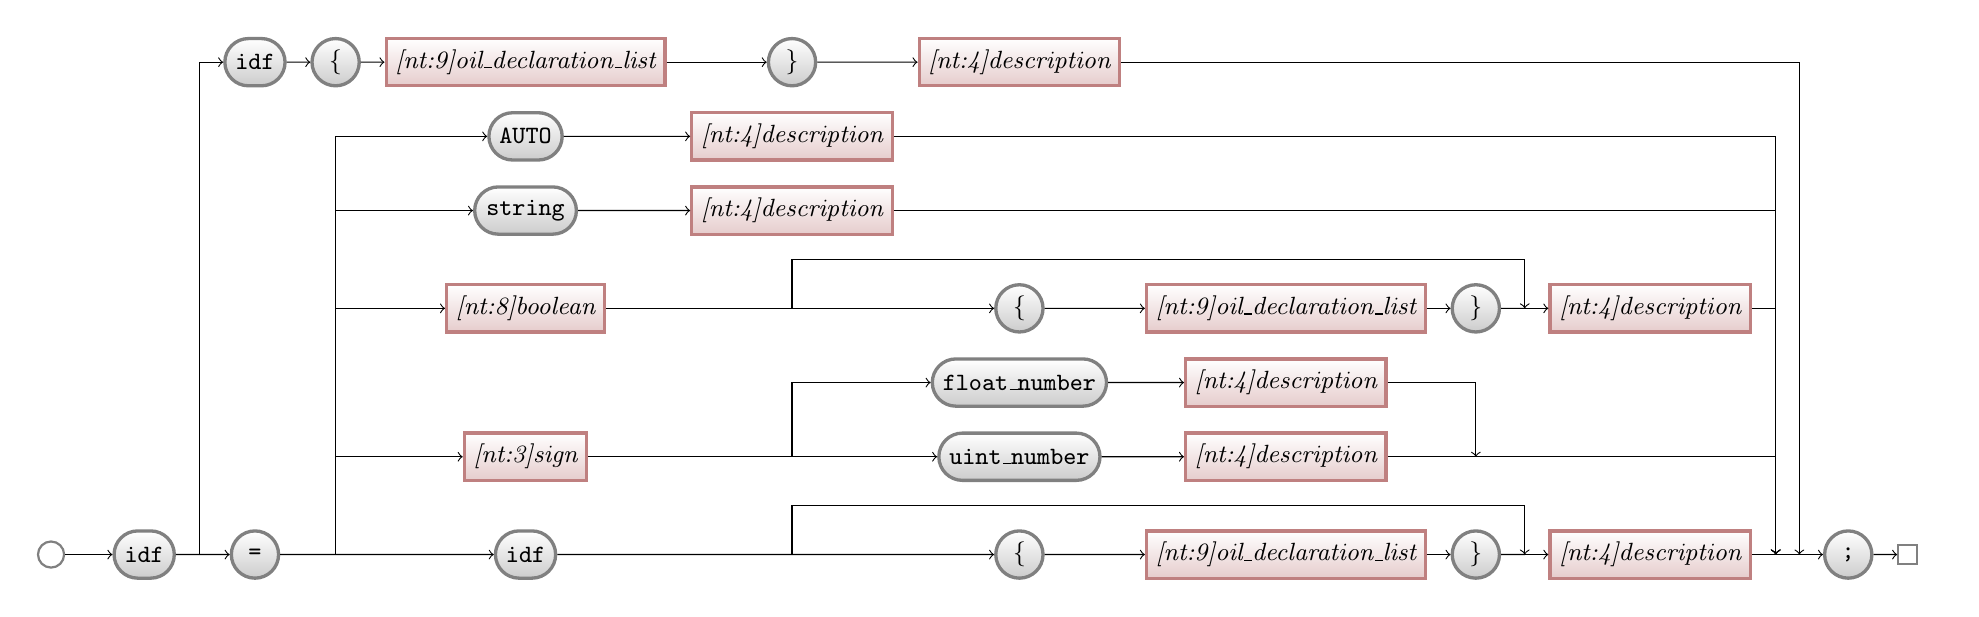
\begin{tikzpicture}
  \matrix[column sep=\ruleMatrixColumnSeparation, row sep=\ruleMatrixRowSeparation] {
    & & & & \node (p8-4) [terminal] {idf}; & \node (p8-5) [terminal] {\{}; & \node (p8-6) [nonterminal] {\nonTerminalSymbol{oil\_declaration\_list}{9}}; & \node (p8-7) [terminal] {\}}; & \node (p8-8) [nonterminal] {\nonTerminalSymbol{description}{4}}; & \\
    & & & & & & \node (p7-6) [terminal] {AUTO}; & \node (p7-7) [nonterminal] {\nonTerminalSymbol{description}{4}}; & \\
    & & & & & & \node (p6-6) [terminal] {string}; & \node (p6-7) [nonterminal] {\nonTerminalSymbol{description}{4}}; & \\
    & & & & & & & & \node (p5-8) [point] {}; & \\
    & & & & & & \node (p4-6) [nonterminal] {\nonTerminalSymbol{boolean}{8}}; & \node (p4-7) [point] {}; & \node (p4-8) [terminal] {\{}; & \node (p4-9) [nonterminal] {\nonTerminalSymbol{oil\_declaration\_list}{9}}; & \node (p4-10) [terminal] {\}}; & \node (p4-11) [point] {}; & \node (p4-12) [nonterminal] {\nonTerminalSymbol{description}{4}}; & \\
    & & & & & & & & \node (p3-8) [terminal] {float\_number}; & \node (p3-9) [nonterminal] {\nonTerminalSymbol{description}{4}}; & \\
    & & & & & & \node (p2-6) [nonterminal] {\nonTerminalSymbol{sign}{3}}; & \node (p2-7) [point] {}; & \node (p2-8) [terminal] {uint\_number}; & \node (p2-9) [nonterminal] {\nonTerminalSymbol{description}{4}}; & \node (p2-10) [point] {}; & \\
    & & & & & & & & \node (p1-8) [point] {}; & \\
    \node (P0start) [firstPoint] {}; & & \node (p0-2) [terminal] {idf}; & \node (p0-3) [point] {}; & \node (p0-4) [terminal] {=}; & \node (p0-5) [point] {}; & \node (p0-6) [terminal] {idf}; & \node (p0-7) [point] {}; & \node (p0-8) [terminal] {\{}; & \node (p0-9) [nonterminal] {\nonTerminalSymbol{oil\_declaration\_list}{9}}; & \node (p0-10) [terminal] {\}}; & \node (p0-11) [point] {}; & \node (p0-12) [nonterminal] {\nonTerminalSymbol{description}{4}}; & \node (p0-13) [point] {}; & \node (p0-14) [point] {}; & \node (p0-15) [terminal] {;}; & \node (p0-16) [lastPoint] {}; & \\
  };
  \draw[->] (P0start) -- (p0-2) ;
  \draw[->] (p0-2) -- (p0-4) ;
  \draw[->] (p0-4) -- (p0-6) ;
  \draw[->] (p0-6) -- (p0-8) ;
  \draw[->] (p0-8) -- (p0-9) ;
  \draw[->] (p0-9) -- (p0-10) ;
  \draw (p0-7) |- (p1-8) ;
  \draw (p0-10) -- (p0-11) ;
  \draw[->] (p1-8) -| (p0-11) ;
  \draw[->] (p0-11) -- (p0-12) ;
  \draw[->] (p0-5) |- (p2-6) ;
  \draw[->] (p2-6) -- (p2-8) ;
  \draw[->] (p2-8) -- (p2-9) ;
  \draw[->] (p2-7) |- (p3-8) ;
  \draw[->] (p3-8) -- (p3-9) ;
  \draw (p2-9) -- (p2-10) ;
  \draw[->] (p3-9) -| (p2-10) ;
  \draw[->] (p0-5) |- (p4-6) ;
  \draw[->] (p4-6) -- (p4-8) ;
  \draw[->] (p4-8) -- (p4-9) ;
  \draw[->] (p4-9) -- (p4-10) ;
  \draw (p4-7) |- (p5-8) ;
  \draw (p4-10) -- (p4-11) ;
  \draw[->] (p5-8) -| (p4-11) ;
  \draw[->] (p4-11) -- (p4-12) ;
  \draw[->] (p0-5) |- (p6-6) ;
  \draw[->] (p6-6) -- (p6-7) ;
  \draw[->] (p0-5) |- (p7-6) ;
  \draw[->] (p7-6) -- (p7-7) ;
  \draw (p0-12) -- (p0-13) ;
  \draw[->] (p2-10) -| (p0-13) ;
  \draw[->] (p4-12) -| (p0-13) ;
  \draw[->] (p6-7) -| (p0-13) ;
  \draw[->] (p7-7) -| (p0-13) ;
  \draw[->] (p0-3) |- (p8-4) ;
  \draw[->] (p8-4) -- (p8-5) ;
  \draw[->] (p8-5) -- (p8-6) ;
  \draw[->] (p8-6) -- (p8-7) ;
  \draw[->] (p8-7) -- (p8-8) ;
  \draw (p0-13) -- (p0-14) ;
  \draw[->] (p8-8) -| (p0-14) ;
  \draw[->] (p0-14) -- (p0-15) ;
  \draw[->] (p0-15) -- (p0-16) ;
\end{tikzpicture}

\nonTerminalSection{oil\_declaration\_list}{9}

\ruleSubsection{goil\_syntax}{goil\_syntax}{244}

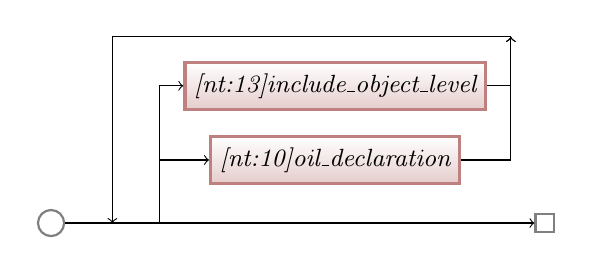
\begin{tikzpicture}
  \matrix[column sep=\ruleMatrixColumnSeparation, row sep=\ruleMatrixRowSeparation] {
    & & & & & & \node (p3-6) [point] {}; & \\
    & & & & & \node (p2-5) [nonterminal] {\nonTerminalSymbol{include\_object\_level}{13}}; & \\
    & & & & & \node (p1-5) [nonterminal] {\nonTerminalSymbol{oil\_declaration}{10}}; & \\
    \node (P0start) [firstPoint] {}; & & \node (p0-2) [point] {}; & \node (p0-3) [point] {}; & \node (p0-4) [point] {}; & & & \node (p0-7) [lastPoint] {}; & \\
  };
  \draw (P0start) -- (p0-3) ;
  \draw[->] (p0-4) |- (p1-5) ;
  \draw[->] (p0-4) |- (p2-5) ;
  \draw[->] (p3-6) -| (p0-2) ;
  \draw[->] (p1-5) -| (p3-6) ;
  \draw[->] (p2-5) -| (p3-6) ;
  \draw[->] (p0-3) -- (p0-7) ;
\end{tikzpicture}

\nonTerminalSection{range}{32}

\ruleSubsection{implementation\_parser}{implementation\_parser}{623}

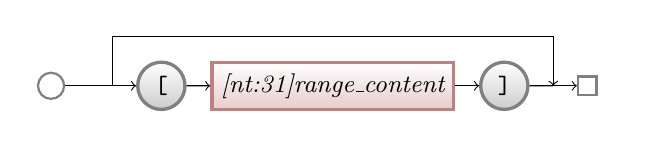
\begin{tikzpicture}
  \matrix[column sep=\ruleMatrixColumnSeparation, row sep=\ruleMatrixRowSeparation] {
    & & & \node (p1-3) [point] {}; & \\
    \node (P0start) [firstPoint] {}; & & \node (p0-2) [point] {}; & \node (p0-3) [terminal] {[}; & \node (p0-4) [nonterminal] {\nonTerminalSymbol{range\_content}{31}}; & \node (p0-5) [terminal] {]}; & \node (p0-6) [point] {}; & \node (p0-7) [lastPoint] {}; & \\
  };
  \draw[->] (P0start) -- (p0-3) ;
  \draw[->] (p0-3) -- (p0-4) ;
  \draw[->] (p0-4) -- (p0-5) ;
  \draw (p0-2) |- (p1-3) ;
  \draw (p0-5) -- (p0-6) ;
  \draw[->] (p1-3) -| (p0-6) ;
  \draw[->] (p0-6) -- (p0-7) ;
\end{tikzpicture}

\nonTerminalSection{range\_content}{31}

\ruleSubsection{implementation\_parser}{implementation\_parser}{583}

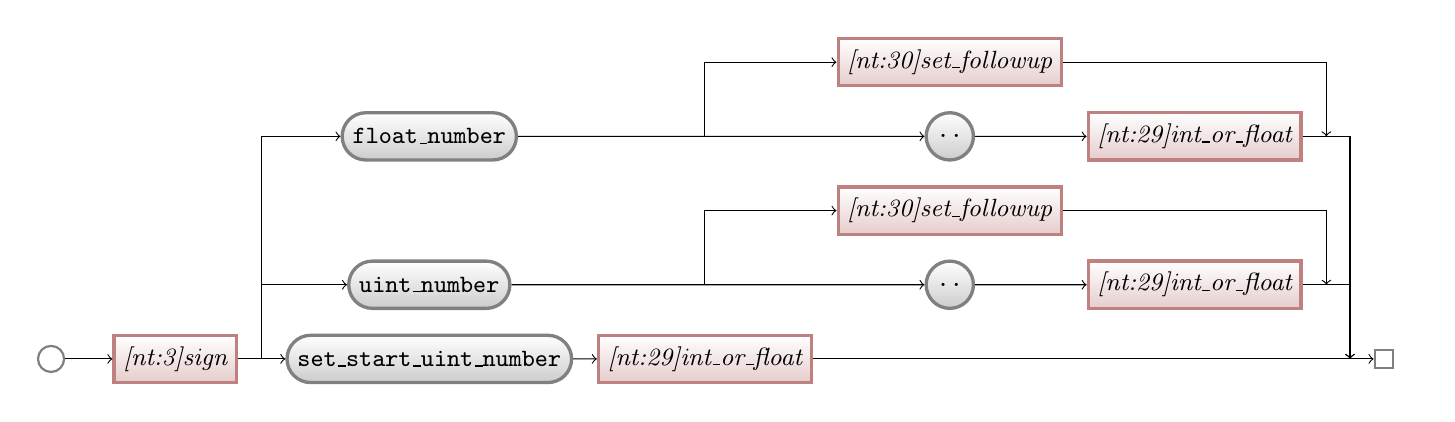
\begin{tikzpicture}
  \matrix[column sep=\ruleMatrixColumnSeparation, row sep=\ruleMatrixRowSeparation] {
    & & & & & & \node (p4-6) [nonterminal] {\nonTerminalSymbol{set\_followup}{30}}; & \\
    & & & & \node (p3-4) [terminal] {float\_number}; & \node (p3-5) [point] {}; & \node (p3-6) [terminal] {..}; & \node (p3-7) [nonterminal] {\nonTerminalSymbol{int\_or\_float}{29}}; & \node (p3-8) [point] {}; & \\
    & & & & & & \node (p2-6) [nonterminal] {\nonTerminalSymbol{set\_followup}{30}}; & \\
    & & & & \node (p1-4) [terminal] {uint\_number}; & \node (p1-5) [point] {}; & \node (p1-6) [terminal] {..}; & \node (p1-7) [nonterminal] {\nonTerminalSymbol{int\_or\_float}{29}}; & \node (p1-8) [point] {}; & \\
    \node (P0start) [firstPoint] {}; & & \node (p0-2) [nonterminal] {\nonTerminalSymbol{sign}{3}}; & \node (p0-3) [point] {}; & \node (p0-4) [terminal] {set\_start\_uint\_number}; & \node (p0-5) [nonterminal] {\nonTerminalSymbol{int\_or\_float}{29}}; & & & & \node (p0-9) [point] {}; & \node (p0-10) [lastPoint] {}; & \\
  };
  \draw[->] (P0start) -- (p0-2) ;
  \draw[->] (p0-2) -- (p0-4) ;
  \draw[->] (p0-4) -- (p0-5) ;
  \draw[->] (p0-3) |- (p1-4) ;
  \draw[->] (p1-4) -- (p1-6) ;
  \draw[->] (p1-6) -- (p1-7) ;
  \draw[->] (p1-5) |- (p2-6) ;
  \draw (p1-7) -- (p1-8) ;
  \draw[->] (p2-6) -| (p1-8) ;
  \draw[->] (p0-3) |- (p3-4) ;
  \draw[->] (p3-4) -- (p3-6) ;
  \draw[->] (p3-6) -- (p3-7) ;
  \draw[->] (p3-5) |- (p4-6) ;
  \draw (p3-7) -- (p3-8) ;
  \draw[->] (p4-6) -| (p3-8) ;
  \draw (p0-5) -- (p0-9) ;
  \draw[->] (p1-8) -| (p0-9) ;
  \draw[->] (p3-8) -| (p0-9) ;
  \draw[->] (p0-9) -- (p0-10) ;
\end{tikzpicture}

\nonTerminalSection{set\_followup}{30}

\ruleSubsection{implementation\_parser}{implementation\_parser}{571}

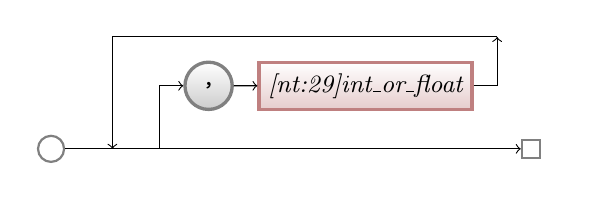
\begin{tikzpicture}
  \matrix[column sep=\ruleMatrixColumnSeparation, row sep=\ruleMatrixRowSeparation] {
    & & & & & & & \node (p2-7) [point] {}; & \\
    & & & & & \node (p1-5) [terminal] {,}; & \node (p1-6) [nonterminal] {\nonTerminalSymbol{int\_or\_float}{29}}; & \\
    \node (P0start) [firstPoint] {}; & & \node (p0-2) [point] {}; & \node (p0-3) [point] {}; & \node (p0-4) [point] {}; & & & & \node (p0-8) [lastPoint] {}; & \\
  };
  \draw (P0start) -- (p0-3) ;
  \draw[->] (p0-4) |- (p1-5) ;
  \draw[->] (p1-5) -- (p1-6) ;
  \draw[->] (p2-7) -| (p0-2) ;
  \draw[->] (p1-6) -| (p2-7) ;
  \draw[->] (p0-3) -- (p0-8) ;
\end{tikzpicture}

\nonTerminalSection{sign}{3}

\ruleSubsection{goil\_syntax}{goil\_syntax}{126}

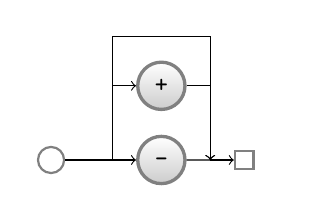
\begin{tikzpicture}
  \matrix[column sep=\ruleMatrixColumnSeparation, row sep=\ruleMatrixRowSeparation] {
    & & & \node (p2-3) [point] {}; & \\
    & & & \node (p1-3) [terminal] {+}; & \\
    \node (P0start) [firstPoint] {}; & & \node (p0-2) [point] {}; & \node (p0-3) [terminal] {-}; & \node (p0-4) [point] {}; & \node (p0-5) [lastPoint] {}; & \\
  };
  \draw[->] (P0start) -- (p0-3) ;
  \draw[->] (p0-2) |- (p1-3) ;
  \draw (p0-2) |- (p2-3) ;
  \draw (p0-3) -- (p0-4) ;
  \draw[->] (p1-3) -| (p0-4) ;
  \draw[->] (p2-3) -| (p0-4) ;
  \draw[->] (p0-4) -- (p0-5) ;
\end{tikzpicture}

\nonTerminalSection{start}{1}

\ruleSubsection{goil\_syntax}{goil\_syntax}{38}

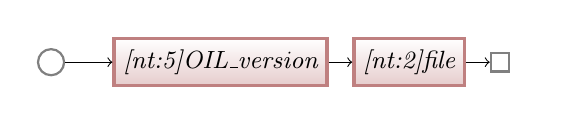
\begin{tikzpicture}
  \matrix[column sep=\ruleMatrixColumnSeparation, row sep=\ruleMatrixRowSeparation] {
    \node (P0start) [firstPoint] {}; & & \node (p0-2) [nonterminal] {\nonTerminalSymbol{OIL\_version}{5}}; & \node (p0-3) [nonterminal] {\nonTerminalSymbol{file}{2}}; & \node (p0-4) [lastPoint] {}; & \\
  };
  \draw[->] (P0start) -- (p0-2) ;
  \draw[->] (p0-2) -- (p0-3) ;
  \draw[->] (p0-3) -- (p0-4) ;
\end{tikzpicture}

\nonTerminalSection{string\_options}{22}

\ruleSubsection{implementation\_parser}{implementation\_parser}{324}

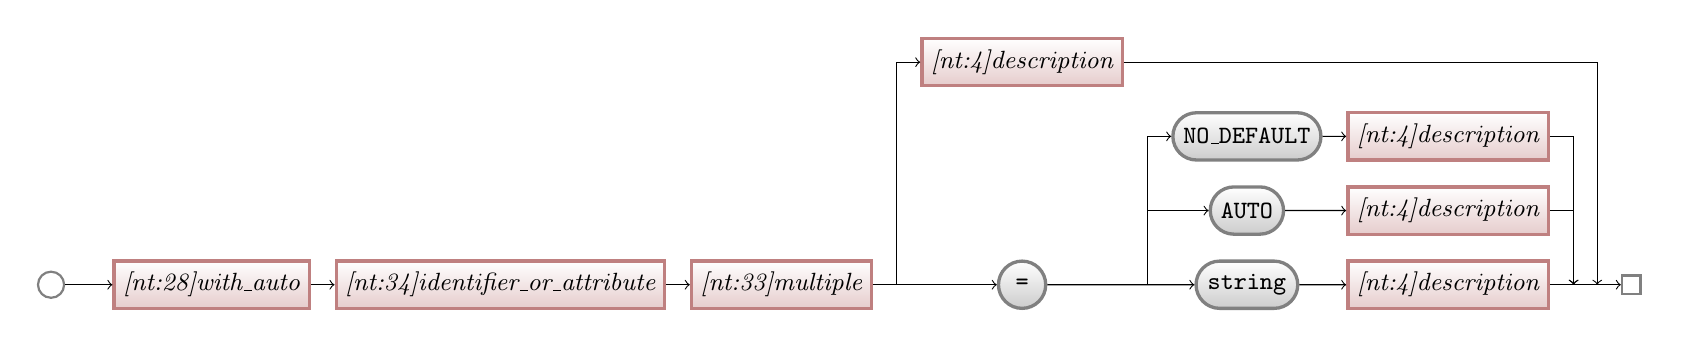
\begin{tikzpicture}
  \matrix[column sep=\ruleMatrixColumnSeparation, row sep=\ruleMatrixRowSeparation] {
    & & & & & & \node (p3-6) [nonterminal] {\nonTerminalSymbol{description}{4}}; & \\
    & & & & & & & & \node (p2-8) [terminal] {NO\_DEFAULT}; & \node (p2-9) [nonterminal] {\nonTerminalSymbol{description}{4}}; & \\
    & & & & & & & & \node (p1-8) [terminal] {AUTO}; & \node (p1-9) [nonterminal] {\nonTerminalSymbol{description}{4}}; & \\
    \node (P0start) [firstPoint] {}; & & \node (p0-2) [nonterminal] {\nonTerminalSymbol{with\_auto}{28}}; & \node (p0-3) [nonterminal] {\nonTerminalSymbol{identifier\_or\_attribute}{34}}; & \node (p0-4) [nonterminal] {\nonTerminalSymbol{multiple}{33}}; & \node (p0-5) [point] {}; & \node (p0-6) [terminal] {=}; & \node (p0-7) [point] {}; & \node (p0-8) [terminal] {string}; & \node (p0-9) [nonterminal] {\nonTerminalSymbol{description}{4}}; & \node (p0-10) [point] {}; & \node (p0-11) [point] {}; & \node (p0-12) [lastPoint] {}; & \\
  };
  \draw[->] (P0start) -- (p0-2) ;
  \draw[->] (p0-2) -- (p0-3) ;
  \draw[->] (p0-3) -- (p0-4) ;
  \draw[->] (p0-4) -- (p0-6) ;
  \draw[->] (p0-6) -- (p0-8) ;
  \draw[->] (p0-8) -- (p0-9) ;
  \draw[->] (p0-7) |- (p1-8) ;
  \draw[->] (p1-8) -- (p1-9) ;
  \draw[->] (p0-7) |- (p2-8) ;
  \draw[->] (p2-8) -- (p2-9) ;
  \draw (p0-9) -- (p0-10) ;
  \draw[->] (p1-9) -| (p0-10) ;
  \draw[->] (p2-9) -| (p0-10) ;
  \draw[->] (p0-5) |- (p3-6) ;
  \draw (p0-10) -- (p0-11) ;
  \draw[->] (p3-6) -| (p0-11) ;
  \draw[->] (p0-11) -- (p0-12) ;
\end{tikzpicture}

\nonTerminalSection{struct\_options}{20}

\ruleSubsection{implementation\_parser}{implementation\_parser}{289}

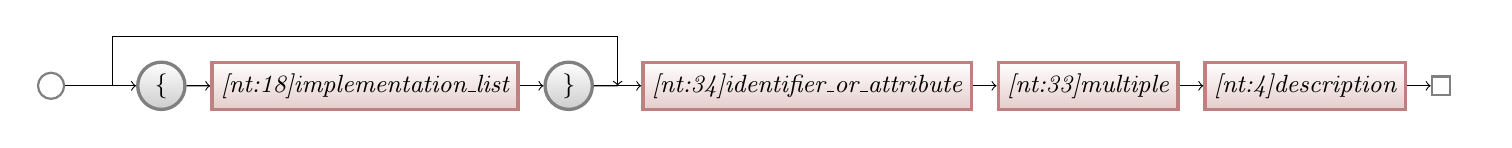
\begin{tikzpicture}
  \matrix[column sep=\ruleMatrixColumnSeparation, row sep=\ruleMatrixRowSeparation] {
    & & & \node (p1-3) [point] {}; & \\
    \node (P0start) [firstPoint] {}; & & \node (p0-2) [point] {}; & \node (p0-3) [terminal] {\{}; & \node (p0-4) [nonterminal] {\nonTerminalSymbol{implementation\_list}{18}}; & \node (p0-5) [terminal] {\}}; & \node (p0-6) [point] {}; & \node (p0-7) [nonterminal] {\nonTerminalSymbol{identifier\_or\_attribute}{34}}; & \node (p0-8) [nonterminal] {\nonTerminalSymbol{multiple}{33}}; & \node (p0-9) [nonterminal] {\nonTerminalSymbol{description}{4}}; & \node (p0-10) [lastPoint] {}; & \\
  };
  \draw[->] (P0start) -- (p0-3) ;
  \draw[->] (p0-3) -- (p0-4) ;
  \draw[->] (p0-4) -- (p0-5) ;
  \draw (p0-2) |- (p1-3) ;
  \draw (p0-5) -- (p0-6) ;
  \draw[->] (p1-3) -| (p0-6) ;
  \draw[->] (p0-6) -- (p0-7) ;
  \draw[->] (p0-7) -- (p0-8) ;
  \draw[->] (p0-8) -- (p0-9) ;
  \draw[->] (p0-9) -- (p0-10) ;
\end{tikzpicture}

\nonTerminalSection{type\_options}{27}

\ruleSubsection{implementation\_parser}{implementation\_parser}{505}

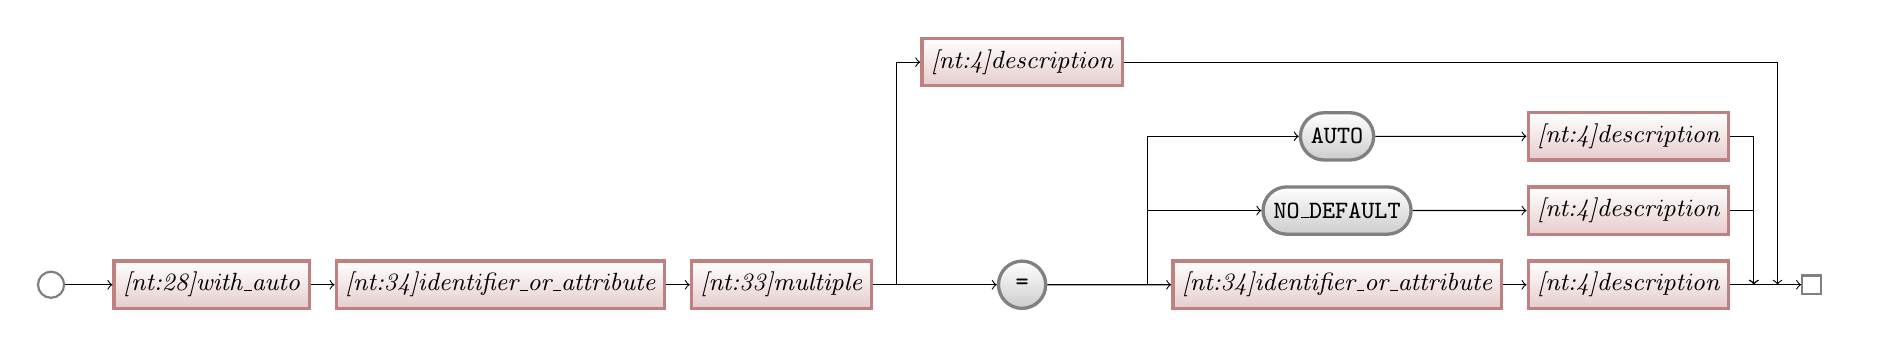
\begin{tikzpicture}
  \matrix[column sep=\ruleMatrixColumnSeparation, row sep=\ruleMatrixRowSeparation] {
    & & & & & & \node (p3-6) [nonterminal] {\nonTerminalSymbol{description}{4}}; & \\
    & & & & & & & & \node (p2-8) [terminal] {AUTO}; & \node (p2-9) [nonterminal] {\nonTerminalSymbol{description}{4}}; & \\
    & & & & & & & & \node (p1-8) [terminal] {NO\_DEFAULT}; & \node (p1-9) [nonterminal] {\nonTerminalSymbol{description}{4}}; & \\
    \node (P0start) [firstPoint] {}; & & \node (p0-2) [nonterminal] {\nonTerminalSymbol{with\_auto}{28}}; & \node (p0-3) [nonterminal] {\nonTerminalSymbol{identifier\_or\_attribute}{34}}; & \node (p0-4) [nonterminal] {\nonTerminalSymbol{multiple}{33}}; & \node (p0-5) [point] {}; & \node (p0-6) [terminal] {=}; & \node (p0-7) [point] {}; & \node (p0-8) [nonterminal] {\nonTerminalSymbol{identifier\_or\_attribute}{34}}; & \node (p0-9) [nonterminal] {\nonTerminalSymbol{description}{4}}; & \node (p0-10) [point] {}; & \node (p0-11) [point] {}; & \node (p0-12) [lastPoint] {}; & \\
  };
  \draw[->] (P0start) -- (p0-2) ;
  \draw[->] (p0-2) -- (p0-3) ;
  \draw[->] (p0-3) -- (p0-4) ;
  \draw[->] (p0-4) -- (p0-6) ;
  \draw[->] (p0-6) -- (p0-8) ;
  \draw[->] (p0-8) -- (p0-9) ;
  \draw[->] (p0-7) |- (p1-8) ;
  \draw[->] (p1-8) -- (p1-9) ;
  \draw[->] (p0-7) |- (p2-8) ;
  \draw[->] (p2-8) -- (p2-9) ;
  \draw (p0-9) -- (p0-10) ;
  \draw[->] (p1-9) -| (p0-10) ;
  \draw[->] (p2-9) -| (p0-10) ;
  \draw[->] (p0-5) |- (p3-6) ;
  \draw (p0-10) -- (p0-11) ;
  \draw[->] (p3-6) -| (p0-11) ;
  \draw[->] (p0-11) -- (p0-12) ;
\end{tikzpicture}

\nonTerminalSection{with\_auto}{28}

\ruleSubsection{implementation\_parser}{implementation\_parser}{544}

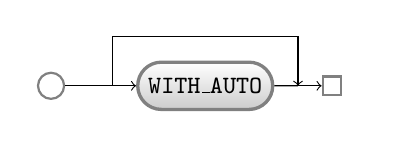
\begin{tikzpicture}
  \matrix[column sep=\ruleMatrixColumnSeparation, row sep=\ruleMatrixRowSeparation] {
    & & & \node (p1-3) [point] {}; & \\
    \node (P0start) [firstPoint] {}; & & \node (p0-2) [point] {}; & \node (p0-3) [terminal] {WITH\_AUTO}; & \node (p0-4) [point] {}; & \node (p0-5) [lastPoint] {}; & \\
  };
  \draw[->] (P0start) -- (p0-3) ;
  \draw (p0-2) |- (p1-3) ;
  \draw (p0-3) -- (p0-4) ;
  \draw[->] (p1-3) -| (p0-4) ;
  \draw[->] (p0-4) -- (p0-5) ;
\end{tikzpicture}



\end{document}
